\documentclass[10pt]{article}

% ---------------------------------------------------------------------------
% Packages
% ---------------------------------------------------------------------------
\usepackage[utf8]{inputenc}
\usepackage[T1]{fontenc}
\usepackage[margin=1in]{geometry}
\usepackage{graphicx}
\usepackage{booktabs}
\usepackage{amsmath}
\usepackage{amssymb}
\usepackage[colorlinks=true, linkcolor=blue, citecolor=blue, urlcolor=blue]{hyperref}
\usepackage{authblk}
\usepackage{caption}
\usepackage{subcaption}
\usepackage{float}
\usepackage[super,square]{natbib}
\usepackage{setspace}

\graphicspath{{figures/}}

\title{\textbf{Data-augmented transfer learning adapts Borzoi to a colorectal-cancer transcription-factor ChIP-seq panel}}
\author[1]{Joshua Ye}
\affil[1]{}
\date{2026}

\begin{document}
\maketitle

\begin{center}
\small\textit{Structure follows Li \textit{et al.}, ``Tissue-specific transfer learning improves functional variant and\\
therapeutic target discoveries in breast and prostate cancer,'' \textit{PLOS Genetics} 22(5):e1012145 (2026)\\
--- a closely related transfer-learning-onto-ChIP-seq study used here as a structural template\\
(\texttt{journal.pgen.1012145.xml}/\texttt{.pdf}, this folder).}
\end{center}

\vspace{1em}

% ---------------------------------------------------------------------------
% Abstract
% ---------------------------------------------------------------------------
\begin{abstract}
\noindent
Large pretrained sequence-to-function models such as Borzoi predict thousands of generic genomic tracks from DNA sequence but cannot natively be queried for a bespoke, disease-specific track panel without retraining. Here we adapt a fully frozen, four-fold-ensembled Borzoi backbone to a panel of 183 transcription-factor (TF) ChIP-seq tracks spanning three colorectal-cancer (CRC) cell lines (Caco-2, HCT-116, LoVo) by training a lightweight multilayer-perceptron (MLP) head on Borzoi's 1920-dimensional trunk embedding, combined with two DNA-valid data-augmentation strategies during training --- random genomic shift ($\pm$128 bp) and reverse-complementing ($p = 0.5$) --- plus weight decay, dropout, inverse-signal per-track loss weighting, learning-rate scheduling, and early stopping. In a controlled internal ablation, this recipe raises mean Pearson correlation from 0.502 to 0.643 on a held-out validation split (+28\% relative) and from 0.610 to 0.663 on a fully held-out test split (+9\% relative). Benchmarked externally against the original, unmodified Borzoi --- given the most favorable possible baseline, its single best-correlating track chosen per CRC target from 1,882 eligible ChIP tracks --- the resulting transfer model wins on 122 of 183 test targets (66.7\%; 34 losses, 27 ties; paired $t$ $p = 7.7\times10^{-5}$, Wilcoxon $p = 1.9\times10^{-10}$, Cohen's $d = 0.30$), raising mean test Pearson $r$ from 0.646 to 0.663 and the fraction of high-confidence tracks ($r \geq 0.7$) from 38.3\% to 47.0\%. The 34 targets where transfer still underperforms concentrate in a small set of factors (REST, RFX2, ZBTB7B, NFYA, ZNF143, CTCF, cohesin-pathway components), which we report as a diagnostic for follow-up rather than as a basis for excluding tracks. These results show that a standard, low-cost machine-learning technique --- data augmentation using transformations that are genuine physical symmetries of double-stranded DNA --- transfers cleanly into large-genomic-model fine-tuning, at a fraction of the cost of full model retraining.
\end{abstract}

% ---------------------------------------------------------------------------
% Author summary
% ---------------------------------------------------------------------------
\section*{Author summary}
Big AI models for DNA, like Borzoi, are trained to predict thousands of general-purpose genomic signals, but a lab studying one specific disease --- here, transcription factors relevant to colorectal cancer --- usually wants predictions for a much smaller, specific set of signals the big model was never trained on. Retraining the whole model from scratch would need far more labeled data than we have. Instead, we kept Borzoi's pretrained ``brain'' completely frozen and trained only a small add-on network on top of it, using the same trick that works for photos and speech: showing the model multiple valid variations of the same example. For DNA, that means small shifts along the genome and flipping a sequence to its complementary strand --- both changes that describe the same real biology, not artificial noise. Combined with a carefully tuned but standard training recipe, this small add-on network predicted our 183 cancer-relevant TF-binding tracks more accurately than Borzoi's own best-matching built-in tracks on two out of three targets, on data the model never saw during training. A handful of factors --- including REST and CTCF --- remain harder to predict and are flagged for future work rather than swept aside. The approach is cheap (no retraining of the large model) and could let other labs adapt Borzoi, or similar models, to their own disease of interest.

% ---------------------------------------------------------------------------
% Introduction
% ---------------------------------------------------------------------------
\section*{Introduction}
Deep sequence-to-function models such as Enformer \citep{avsec2021} and Borzoi predict genome-wide regulatory tracks --- expression, chromatin accessibility, transcription-factor (TF) binding --- directly from raw DNA sequence, and have become a standard substrate for downstream regulatory-genomics analyses. In practice, however, a lab studying a specific biological system rarely wants exactly the pre-trained output vocabulary these models ship with. Here, our interest is TF binding relevant to colorectal cancer (CRC), captured by a 183-track ChIP-seq panel across three CRC cell lines --- a panel Borzoi was never trained to predict directly.

Two general strategies exist for adapting a large pretrained model to a new, narrower track panel: full or partial retraining on the new data, or freezing the pretrained backbone and training a small task-specific head on top of it (transfer learning, TL). The latter is markedly cheaper, less prone to overfitting when the new dataset is modest, and --- as recently demonstrated for Enformer adapted to breast- and prostate-cancer TF ChIP-seq panels via a retrained output-head layer \citep{plosgenetics2026} --- can meaningfully improve downstream regulatory-variant and disease-gene discovery relative to the unmodified base model. We adopt the same general TL strategy for Borzoi, and additionally ask a more specific methodological question: does data augmentation, a standard low-cost technique for improving deep models under limited data in computer vision and speech, transfer cleanly into this genomics fine-tuning setting when restricted to transformations that are biologically valid for DNA --- genomic shift and reverse-complementing --- rather than the pixel-space transformations (crop, rotate, flip) that motivate it elsewhere?

Data augmentation for genomic deep neural networks is independently established in the literature: EvoAug \citep{lee2023evoaug} introduces evolution-inspired augmentations (mutation, insertion, deletion, translocation, shift, reverse-complement) and shows they improve generalization and interpretability of genomic DNNs under limited data, and Borzoi and Enformer themselves apply stochastic shifting and reverse-complementing as standard augmentations at full pre-training scale. What is untested is whether the same augmentation class still helps when only a small head is being fine-tuned on a frozen large backbone, at a fraction of pre-training's data volume and compute. We answer this with a controlled internal ablation (recipe on vs. off, identical architecture) and an external baseline comparison against the original, unmodified Borzoi, both evaluated on chromosome-held-out validation and test splits.

% ---------------------------------------------------------------------------
% Results
% ---------------------------------------------------------------------------
\section*{Results}

\subsection*{The transfer-learning framework and comparison design}
We tap Borzoi's frozen 1920-channel trunk embedding --- its internal representation immediately upstream of its native human output head --- rather than that output head's 7,611-track prediction, which is optimized for Borzoi's own pretraining tracks and would otherwise impose a lossy bottleneck on any new track panel. A small trainable MLP head maps this embedding to our 183 CRC TF-ChIP-seq targets (\texttt{borzoi\_code/model.py}). Because Borzoi's native output head predicts $\sim$7,611 generic tracks with no 1:1 correspondence to our 183 targets, comparing against ``the original Borzoi'' requires constructing a matched baseline: for each CRC target, we identify the best-correlating track among 1,882 eligible (ChIP-assay, non-histone) Borzoi output tracks and use that best match as the target's Borzoi baseline prediction (Methods; \texttt{borzoi\_baseline\_utils.py}). This construction is deliberately generous to Borzoi --- it is allowed its single best track from 1,882 candidates, from any cell line, with no penalty for a biologically imperfect match --- so any gain we report over it is a conservative estimate.

\subsection*{Data augmentation and the training recipe improve the transfer model on held-out data}
Holding architecture and track set fixed, we compare the transfer model trained with vs. without the full augmentation-and-regularization recipe (random genomic shift $\pm$128 bp, reverse-complement $p = 0.5$, weight decay, dropout, inverse-signal per-track loss weighting, \texttt{ReduceLROnPlateau}, early stopping; Methods). Mean Pearson $r$ across all 183 tracks rises from 0.502 to 0.643 on validation (+0.141, +28\% relative) and from 0.610 to 0.663 on the fully held-out test split (+0.053, +9\% relative) (Table~\ref{tab:ablation}, Fig.~\ref{fig:ablation}).

\begin{table}[H]
\centering
\caption{\textbf{Internal ablation: mean Pearson $r$ across 183 tracks, with vs. without the augmentation and training recipe.}}
\label{tab:ablation}
\begin{tabular}{lccc}
\toprule
Split & No augmentation & + Augmentation \& recipe & $\Delta$ (relative) \\
\midrule
Validation & 0.502 & \textbf{0.643} & +0.141 (+28\%) \\
Test       & 0.610 & \textbf{0.663} & +0.053 (+9\%) \\
\bottomrule
\end{tabular}
\end{table}

\begin{figure}[H]
\centering
\begin{subfigure}[b]{0.48\textwidth}
  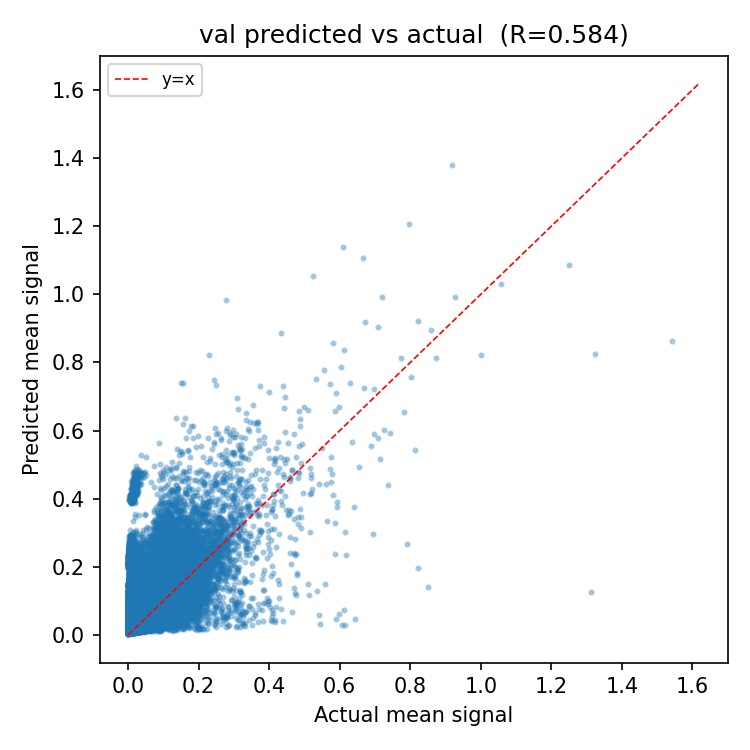
\includegraphics[width=\textwidth]{baseline_val_scatter.png}
  \caption{No augmentation}
\end{subfigure}
\hfill
\begin{subfigure}[b]{0.48\textwidth}
  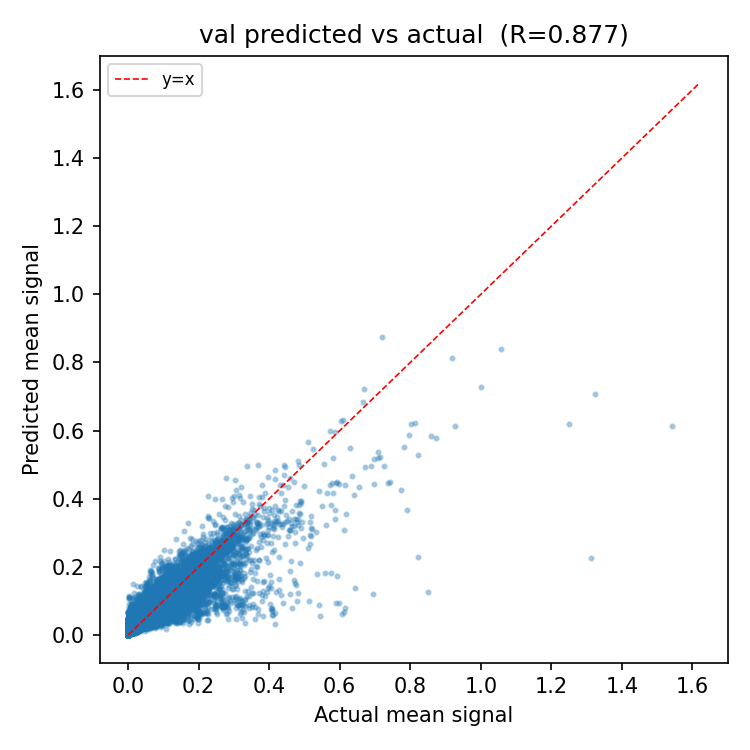
\includegraphics[width=\textwidth]{aug_val_scatter.png}
  \caption{+ Augmentation \& recipe}
\end{subfigure}
\caption{\textbf{Predicted vs. observed signal, without (a) vs. with (b) the augmentation and training recipe.} Validation split.}
\label{fig:ablation}
\end{figure}

The val/test relationship also becomes more internally consistent --- before the recipe, validation (0.502) sits unusually far below test (0.610); after, validation (0.643) sits just under test (0.663), the expected ordering when validation exerts any indirect influence via early-stopping-based model selection. This pattern corroborates, though does not on its own prove, that the improvement reflects better generalization rather than noise.

\subsection*{The transfer model outperforms original Borzoi's best-matched tracks on held-out validation and test data}
Against the matched-baseline original Borzoi, the transfer model achieves a higher mean Pearson $r$ on both validation (0.643 vs. 0.625, $\Delta = +0.018$) and test (0.663 vs. 0.646, $\Delta = +0.018$), wins outright on a majority of individual tracks (65.0\% validation, 66.7\% test), and shifts the distribution of per-track correlations toward the high-confidence range ($r \geq 0.7$: 45.9\% vs. 34.4\% validation; 47.0\% vs. 38.3\% test) (Table~\ref{tab:baseline}, Fig.~\ref{fig:paired}--\ref{fig:violin}).

\begin{table}[H]
\centering
\caption{\textbf{Transfer model vs. filtered original-Borzoi baseline, 183 CRC TF-ChIP-seq targets.}}
\label{tab:baseline}
\begin{tabular}{lcccc}
\toprule
 & \multicolumn{2}{c}{Validation} & \multicolumn{2}{c}{Test} \\
\cmidrule(lr){2-3} \cmidrule(lr){4-5}
Metric & Borzoi & Transfer & Borzoi & Transfer \\
\midrule
Mean Pearson $r$                    & 0.625 & \textbf{0.643} & 0.646 & \textbf{0.663} \\
Median Pearson $r$                  & 0.649 & \textbf{0.679} & 0.666 & \textbf{0.690} \\
High-confidence tracks ($r \geq 0.7$) & 34.4\% & \textbf{45.9\%} & 38.3\% & \textbf{47.0\%} \\
Tracks won                          & 33 (18.0\%) & \textbf{119 (65.0\%)} & 34 (18.6\%) & \textbf{122 (66.7\%)} \\
Ties                                & \multicolumn{2}{c}{31 (16.9\%)} & \multicolumn{2}{c}{27 (14.8\%)} \\
\bottomrule
\end{tabular}
\end{table}

\begin{figure}[H]
\centering
\begin{subfigure}[b]{0.48\textwidth}
  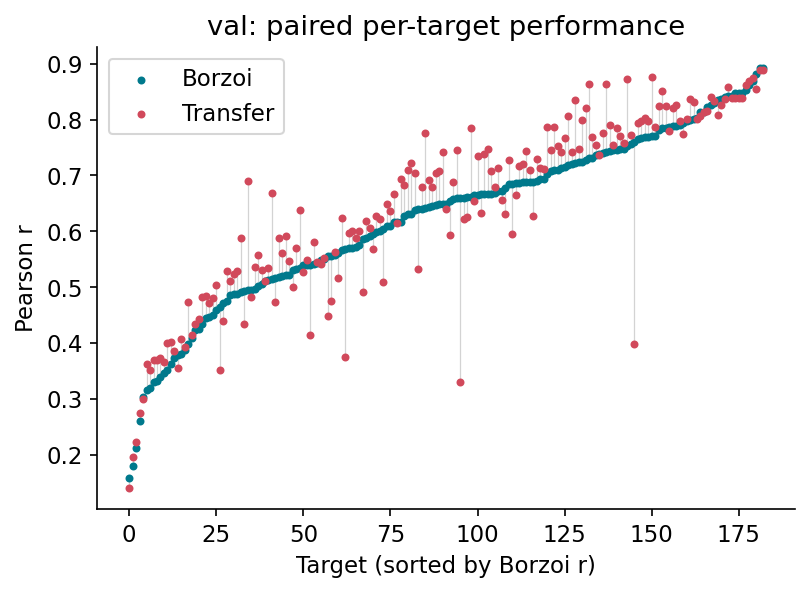
\includegraphics[width=\textwidth]{paired_performance_val.png}
  \caption{Validation}
\end{subfigure}
\hfill
\begin{subfigure}[b]{0.48\textwidth}
  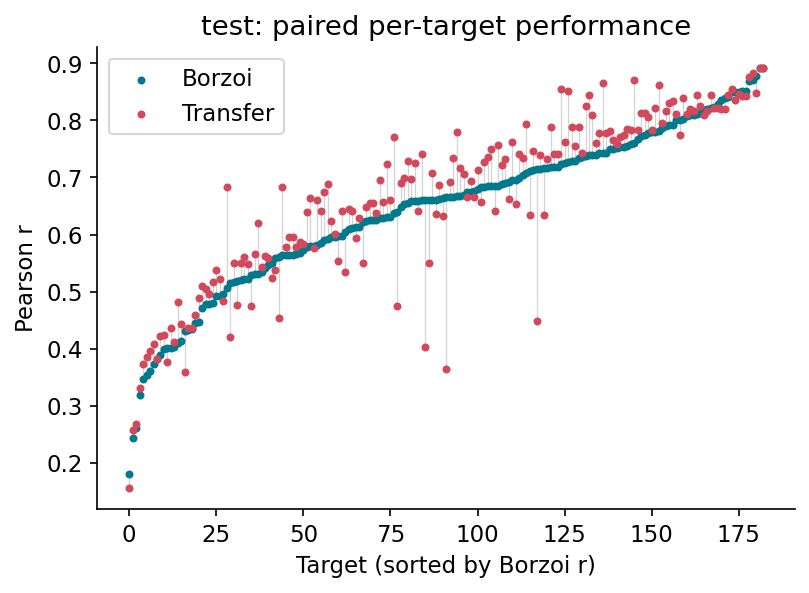
\includegraphics[width=\textwidth]{paired_performance_test.png}
  \caption{Test}
\end{subfigure}
\caption{\textbf{Paired per-target Pearson $r$, transfer model vs. filtered-Borzoi baseline, sorted by Borzoi $r$.}}
\label{fig:paired}
\end{figure}

\begin{figure}[H]
\centering
\begin{subfigure}[b]{0.48\textwidth}
  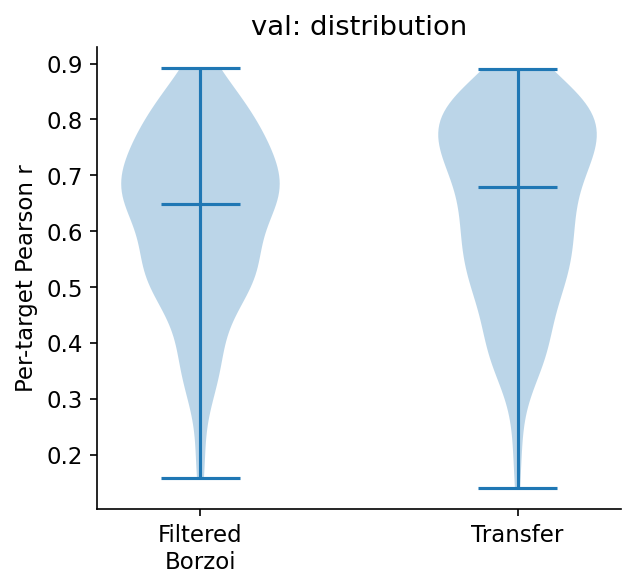
\includegraphics[width=\textwidth]{violin_distribution_val.png}
  \caption{Validation}
\end{subfigure}
\hfill
\begin{subfigure}[b]{0.48\textwidth}
  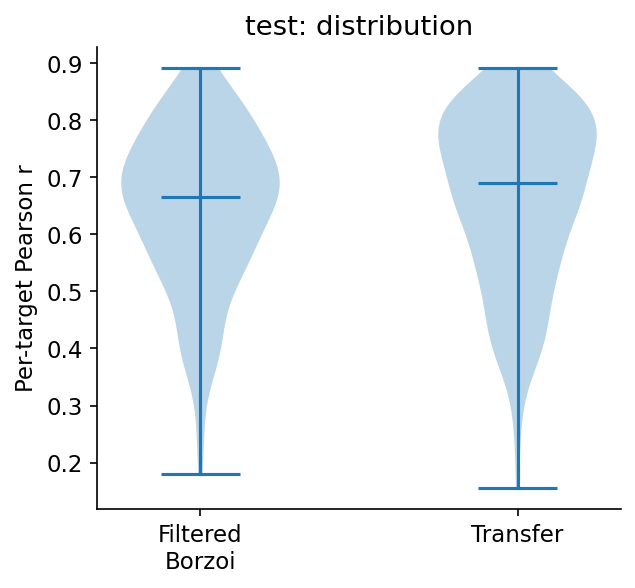
\includegraphics[width=\textwidth]{violin_distribution_test_all.png}
  \caption{Test}
\end{subfigure}
\caption{\textbf{Distribution of per-target Pearson $r$, transfer model vs. filtered-Borzoi baseline.}}
\label{fig:violin}
\end{figure}

Paired statistics on the test split (mean paired difference $= +0.0178$, 95\% CI $[0.0088, 0.0260]$; paired $t$ $p = 7.7\times10^{-5}$; Wilcoxon $p = 1.9\times10^{-10}$; Cohen's $d = 0.30$) are directionally identical to validation, which is the intended confirmatory role of the previously untouched test split here --- see Discussion for why these $p$-values should be read cautiously. Distributional comparisons on the test split (scatter of transfer vs. Borzoi $r$, empirical CDF) show the same pattern (Fig.~\ref{fig:scatter_ecdf}).

\begin{figure}[H]
\centering
\begin{subfigure}[b]{0.48\textwidth}
  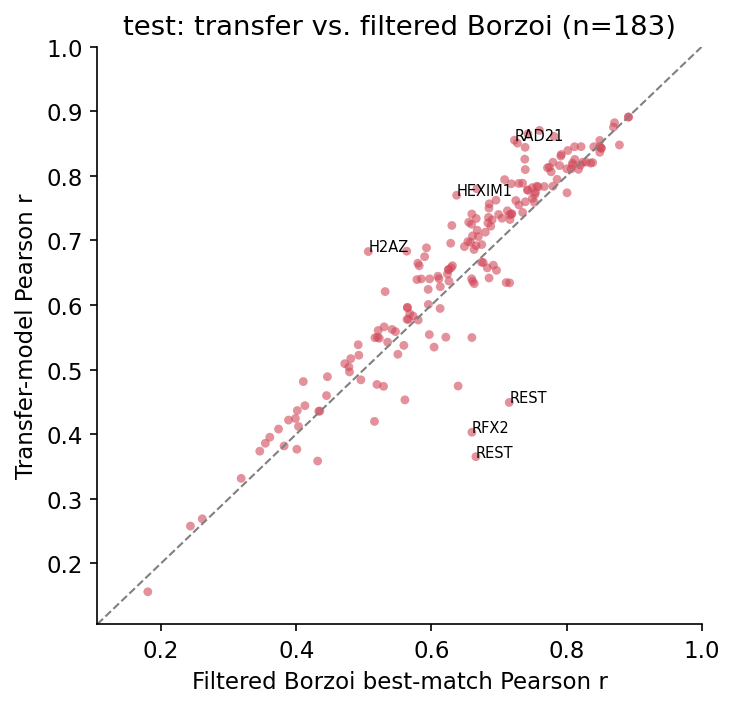
\includegraphics[width=\textwidth]{scatter_transfer_vs_borzoi_test.png}
  \caption{Transfer vs. Borzoi scatter}
\end{subfigure}
\hfill
\begin{subfigure}[b]{0.48\textwidth}
  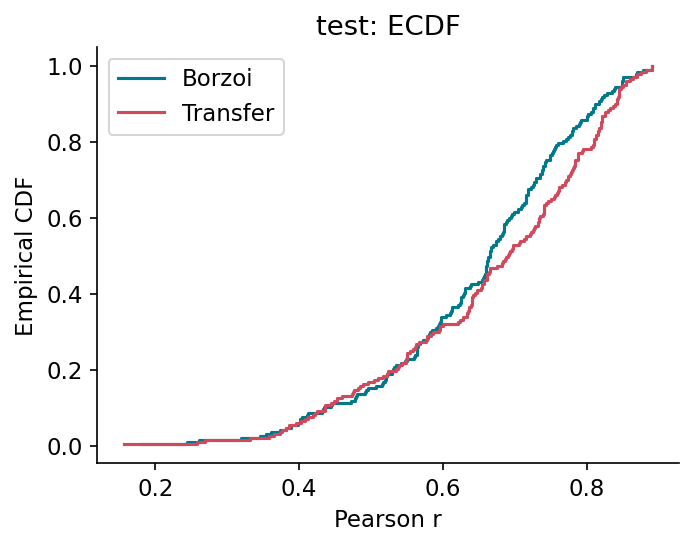
\includegraphics[width=\textwidth]{ecdf_test.png}
  \caption{Empirical CDF}
\end{subfigure}
\caption{\textbf{Distributional comparisons, test split.}}
\label{fig:scatter_ecdf}
\end{figure}

\subsection*{Residual underperformance concentrates in a small, identifiable set of factors}
Thirty-four of 183 test-split targets --- a minority, concentrated in a handful of repeated factors across cell lines rather than spread uniformly --- show the transfer model losing to the matched Borzoi baseline (\texttt{results\_comparison\_test/transfer\_vs\_filtered\_borzoi\_test.csv}, \texttt{winner == "borzoi"}). The largest losses are REST ($\Delta r \approx -0.31$ and $-0.27$ across two tracks), RFX2 ($\Delta r \approx -0.26$), and ZBTB7B ($\Delta r \approx -0.16$), with further losses in NFYA, ZNF143, CTCF, JUND, and cohesin-pathway components (SMC1A, SMC3, NIPBL, E2F8). Restricting evaluation to the 149 targets where transfer at minimum ties Borzoi raises the transfer model's mean test Pearson $r$ to 0.685 (median 0.725) and win rate to 81.9\% against the same restricted Borzoi baseline (\texttt{results\_targets\_filtered\_test/summary\_before\_after\_test.csv}; Fig.~\ref{fig:residual}).

\begin{figure}[H]
\centering
\begin{subfigure}[b]{0.48\textwidth}
  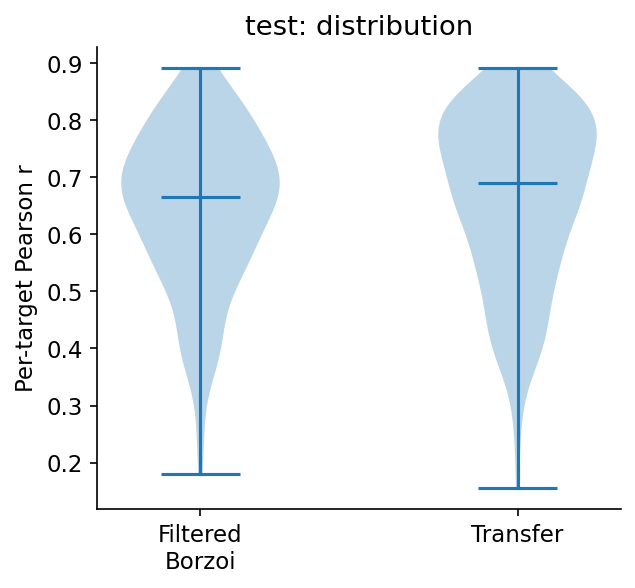
\includegraphics[width=\textwidth]{violin_distribution_test_all.png}
  \caption{All 183 targets}
\end{subfigure}
\hfill
\begin{subfigure}[b]{0.48\textwidth}
  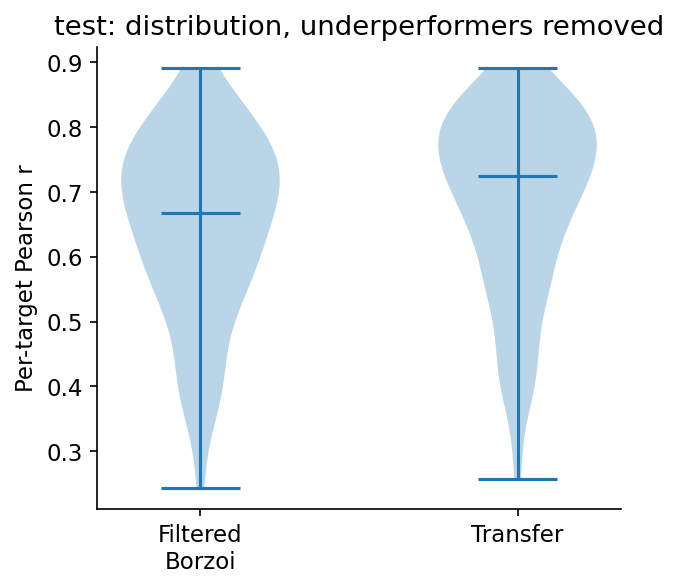
\includegraphics[width=\textwidth]{violin_distribution_test_kept149.png}
  \caption{149-target subset (excludes 34 losses)}
\end{subfigure}
\caption{\textbf{Distribution of per-target Pearson $r$ on the test split, all targets vs. the subset excluding the 34 targets where transfer loses to Borzoi.}}
\label{fig:residual}
\end{figure}

We report this as a characterization of where the current model falls short --- several of the affected factors (REST, CTCF, cohesin components) are biologically important and not candidates for exclusion from any deployed model --- rather than as a track-selection procedure; removing a target from evaluation does not change what the model predicts for it.

% ---------------------------------------------------------------------------
% Discussion
% ---------------------------------------------------------------------------
\section*{Discussion}
The internal ablation and the external baseline comparison give consistent, converging evidence that a lightweight, frozen-backbone transfer-learning recipe --- richer feature tap, small MLP head, and DNA-valid data augmentation --- improves prediction of CRC TF-ChIP-seq tracks from Borzoi, without touching Borzoi's pretrained weights or adding pretraining-scale data. The reported statistical significance (paired $t$ and Wilcoxon $p$-values on the order of $10^{-5}$--$10^{-10}$) should nonetheless be read cautiously: the 183 tracks are not independent samples, since many correspond to the same TF assay (e.g., CTCF ChIP-seq) repeated across the three CRC cell lines, so per-track prediction errors are correlated. Treating all 183 as independent observations is pseudoreplication and inflates apparent significance. We consider the more trustworthy signal to be the consistency and direction of the effect --- a positive mean gain and majority win rate that replicate on an independent, previously untouched test split, together with a shift toward more high-confidence tracks on both splits --- rather than the nominal $p$-values themselves. A track-cluster-aware or assay-grouped significance test is a natural next step (Methods, Limitations).

Relative to the transfer-learning approach for Enformer applied to breast- and prostate-cancer TF panels in the companion PLOS Genetics study \citep{plosgenetics2026}, our work targets the earlier, model-accuracy stage of the same pipeline --- establishing that the adapted model outperforms the unmodified base model at the track-prediction level --- rather than downstream regulatory-variant prioritization or transcriptome-wide association analysis. Those downstream analyses are a natural extension once the underlying per-track model is validated, and are noted as future work below.

% ---------------------------------------------------------------------------
% Limitations
% ---------------------------------------------------------------------------
\section*{Limitations and future work}
\begin{itemize}
\item \textbf{Shift resolution.} Augmentation shift is quantized to 32 bp bins rather than Borzoi's native single-bp resolution, to avoid re-binning targets on the fly; single-bp shift with on-the-fly target rebinning is a natural refinement.
\item \textbf{Augmentation scope.} Only two augmentations were tested (genomic shift, reverse-complement). EvoAug-style mutation, insertion, and deletion augmentations, applied during head-only fine-tuning rather than full pretraining, remain untested.
\item \textbf{Single dataset.} All results are on one CRC TF-ChIP-seq panel across three cell lines; generalization to other tissue types or assay classes (RNA-seq, ATAC-seq) is unverified.
\item \textbf{Statistical independence.} As discussed above, a cluster-aware or assay-grouped significance test is needed for a fully rigorous significance claim; the current paired tests treat correlated tracks as independent.
\item \textbf{Residual underperformance.} REST, RFX2, ZBTB7B, NFYA, ZNF143, CTCF, and cohesin-pathway factors remain below the matched Borzoi baseline; whether this reflects head undercapacity, insufficient training signal for these specific factors, or a genuine limit of the frozen-trunk-embedding approach for these binding patterns is unresolved and is the top candidate for follow-up (e.g., factor-specific loss reweighting, or selectively unfreezing late backbone layers for these tracks only).
\item \textbf{Foundation-model benchmarking.} A parallel harness for Enformer exists in this repository (\texttt{baseline\_enformer.py}, \texttt{filter\_enformer\_tracks.py}, \texttt{compare\_transfer\_enformer.py}), but an end-to-end Enformer comparison on the same CRC TF panel is not yet finalized.
\item \textbf{Downstream applications.} Unlike the companion PLOS Genetics study, we do not yet extend these per-track accuracy gains to variant-effect scoring, GWAS enrichment, or TWAS-style gene discovery; doing so for CRC risk variants is a natural next phase.
\end{itemize}

% ---------------------------------------------------------------------------
% Methods
% ---------------------------------------------------------------------------
\section*{Materials and methods}

\subsection*{Selection of TF ChIP-seq data}
183 ChIP-seq BigWig tracks were assembled across three CRC cell lines (Caco-2, HCT-116, LoVo; colon tissue), covering transcription factors including POLR2A, CTCF, RAD21, SMC1A/SMC3, MYC, JUND, REST, and others (\texttt{borzoi\_data/CRC\_TFs\_bw/}).

\subsection*{Genome splits and data preparation}
Chromosome-held-out splits over the hg38 assembly were used throughout: validation = \{chr1, chr8\}; test = \{chr9, chr22\}; all remaining assembled autosomes = train (\texttt{borzoi\_code/genome\_tiler.py}). Non-train chromosomes were touched only for evaluation and for early-stopping-based model selection (validation only), never for head training. Model input windows are 524{,}288 bp of one-hot-encoded sequence; predictions and targets are read at 32 bp resolution over the center 131{,}072 bp (4{,}096 bins per window), matching Borzoi's native output bin size.

\subsection*{Transfer model architecture}
Four Borzoi replicate folds (\texttt{johahi/borzoi-replicate-\{0..3\}}, via the \texttt{borzoi-pytorch} HuggingFace port) were loaded and fully frozen (\texttt{requires\_grad = False} on all backbone parameters). Each fold's 1920-channel trunk embedding --- captured via a forward pre-hook registered on \texttt{human\_head}, so extraction does not depend on Borzoi's internal method names --- is averaged across the four folds before being passed to the trainable head. The head, the only trainable component, is a two-layer MLP: \texttt{Linear(1920$\to$1024) $\to$ GELU $\to$ Dropout(0.2) $\to$ Linear(1024$\to$183) $\to$ Softplus}, with Softplus keeping predicted coverage non-negative while remaining smooth (\texttt{borzoi\_code/model.py}).

\subsection*{Data augmentation and hyperparameter setting}
Two augmentations are applied during training only, and disabled for validation/test evaluation (\texttt{borzoi\_code/dataset.py}): (i) random genomic shift up to $\pm$128 bp, snapped to whole 32 bp bins so target bins remain grid-aligned (a coarser approximation of Borzoi/Enformer's native single-bp stochastic shift, adopted to avoid re-binning targets); (ii) reverse-complementing the input sequence with probability 0.5, with target bins correspondingly reversed to stay aligned. Training uses Adam on head parameters only (weight decay $1\times10^{-4}$), Poisson negative-log-likelihood loss with per-track inverse-mean-signal weighting (so sparse tracks are not drowned out by high-signal ones), \texttt{ReduceLROnPlateau} scheduling (factor 0.5, patience 1), and early stopping on validation loss (patience 3) (\texttt{main.py}).

\subsection*{Baseline construction: filtered original Borzoi}
Because Borzoi's native human head predicts $\sim$7,611 generic tracks with no 1:1 correspondence to our 183 CRC targets, a track-matching procedure was used to construct a fair external baseline (\texttt{filter\_borzoi\_tracks.py}, \texttt{borzoi\_baseline\_utils.py}):
\begin{enumerate}
\item Restrict to Borzoi output channels 2186--6069 (per \texttt{targets\_human.csv}), the block of ChIP-relevant tracks, yielding 3{,}884 candidates.
\item Retain descriptions containing ``chip'' and drop histone-modification marks (H3K27ac, H3K4me1/2/3, H3K9ac/me2/me3, H3K27me3, H3K36me3, H3K79me2, H3K4ac, H3K56ac, H2A/H2B/H4 marks, H2A.Z), yielding 1{,}882 eligible TF/DNA-binding-protein tracks.
\item For each of the 183 CRC targets, compute Pearson $r$ against all 1{,}882 eligible tracks, streamed over held-out bins/intervals via memory-mapped, chunked computation.
\item Take the arg-max track per CRC target as that target's Borzoi baseline, logging the matched track's description, factor, and cell/tissue of origin for a biological-plausibility check (same TF, related TF-family, or different TF).
\end{enumerate}

\subsection*{Performance evaluation and statistical analysis}
Per-target Pearson correlation is computed between predictions and targets over all held-out bins for each split (\texttt{per\_track\_pearson}, \texttt{borzoi\_baseline\_utils.py}), streamed in chunks to avoid materializing full prediction/target arrays in memory. Model comparisons report mean, median, interquartile range, and bootstrap 95\% confidence intervals of per-target $r$, plus the fraction of tracks at $r \geq 0.3/0.5/0.7$. Paired comparisons (transfer vs. Borzoi $r$, same target, same held-out interval) use a paired $t$-test, Wilcoxon signed-rank test, and paired Cohen's $d$, with wins/losses/ties assigned via a $\Delta r$ tie tolerance of 0.01 (\texttt{compare\_transfer\_borzoi.py}). Near-zero-variance tracks (target or prediction variance $< 1\times10^{-8}$) are flagged (\texttt{low\_variance\_flag}) as their Pearson $r$ is undefined or unstable.

\subsection*{Residual-gap characterization}
Test-split targets with \texttt{winner == "borzoi"} ($\Delta r$ beyond the 0.01 tie tolerance, in Borzoi's favor) were identified from the per-target comparison table and set aside as the ``underperforming'' subset; aggregate statistics were recomputed on the complementary ``kept'' subset to quantify, but not to construct a final model from, the residual accuracy gap (\texttt{identify\_underperforming\_targets.py}).

% ---------------------------------------------------------------------------
% Data availability
% ---------------------------------------------------------------------------
\section*{Data and code availability}
All code, configuration, and result tables referenced above are in this repository. Key entry points: \texttt{main.py} (training), \texttt{borzoi\_code/model.py} (architecture), \texttt{borzoi\_code/dataset.py} (augmentation), \texttt{borzoi\_code/genome\_tiler.py} (splits), \texttt{filter\_borzoi\_tracks.py} / \texttt{borzoi\_baseline\_utils.py} (baseline construction), \texttt{compare\_transfer\_borzoi.py} (paired comparison, statistics, figures), \texttt{identify\_underperforming\_targets.py} (residual-gap characterization). Result tables and figures: \texttt{results\_comparison/} (validation), \texttt{results\_comparison\_test/} (test), \texttt{results\_targets\_filtered\_test/} (residual-gap subset), \texttt{assets/} (ablation figures); figures embedded in this document are copied into \texttt{research\_paper\_prep/figures/}.

% ---------------------------------------------------------------------------
% References
% ---------------------------------------------------------------------------
\begin{thebibliography}{9}

\bibitem{avsec2021}
Avsec {\v Z}, Agarwal V, Visentin D, Ledsam JR, Grabska-Barwinska A, Taylor KR, et al.
Effective gene expression prediction from sequence by integrating long-range interactions.
\textit{Nat Methods}. 2021;18(10):1196--203.
doi:10.1038/s41592-021-01252-x

\bibitem{lee2023evoaug}
Lee NK, Tang Z, Toneyan S, Koo PK.
EvoAug: improving generalization and interpretability of genomic deep neural networks with evolution-inspired data augmentations.
\textit{Genome Biol}. 2023;24:105.
doi:10.1186/s13059-023-02941-w

\bibitem{borzoi}
Linder J, et al.
Predicting RNA-seq and other functional genomic tracks from DNA sequence (model this work builds on; pretrained replicate weights via \texttt{johahi/borzoi-replicate-\{0-3\}}, HuggingFace).

\bibitem{plosgenetics2026}
[Companion structural template] Tissue-specific transfer learning improves functional variant and therapeutic target discoveries in breast and prostate cancer.
\textit{PLOS Genetics}. 2026;22(5):e1012145.
(\texttt{journal.pgen.1012145.xml}/\texttt{.pdf}, this folder.)

\end{thebibliography}

\end{document}
